%T4.2 TUD 3PM
%Summary: 
%In collaboration with JSI, TUD studied whether supporting contacts
%in human arm reaching tasks are planned or an effect of a reactive controller. 
%Probabilistic inference in learned models of kinematics provide evidence for planned contacts in human reaching. 

%description of work:
\begin{figure}
\centering
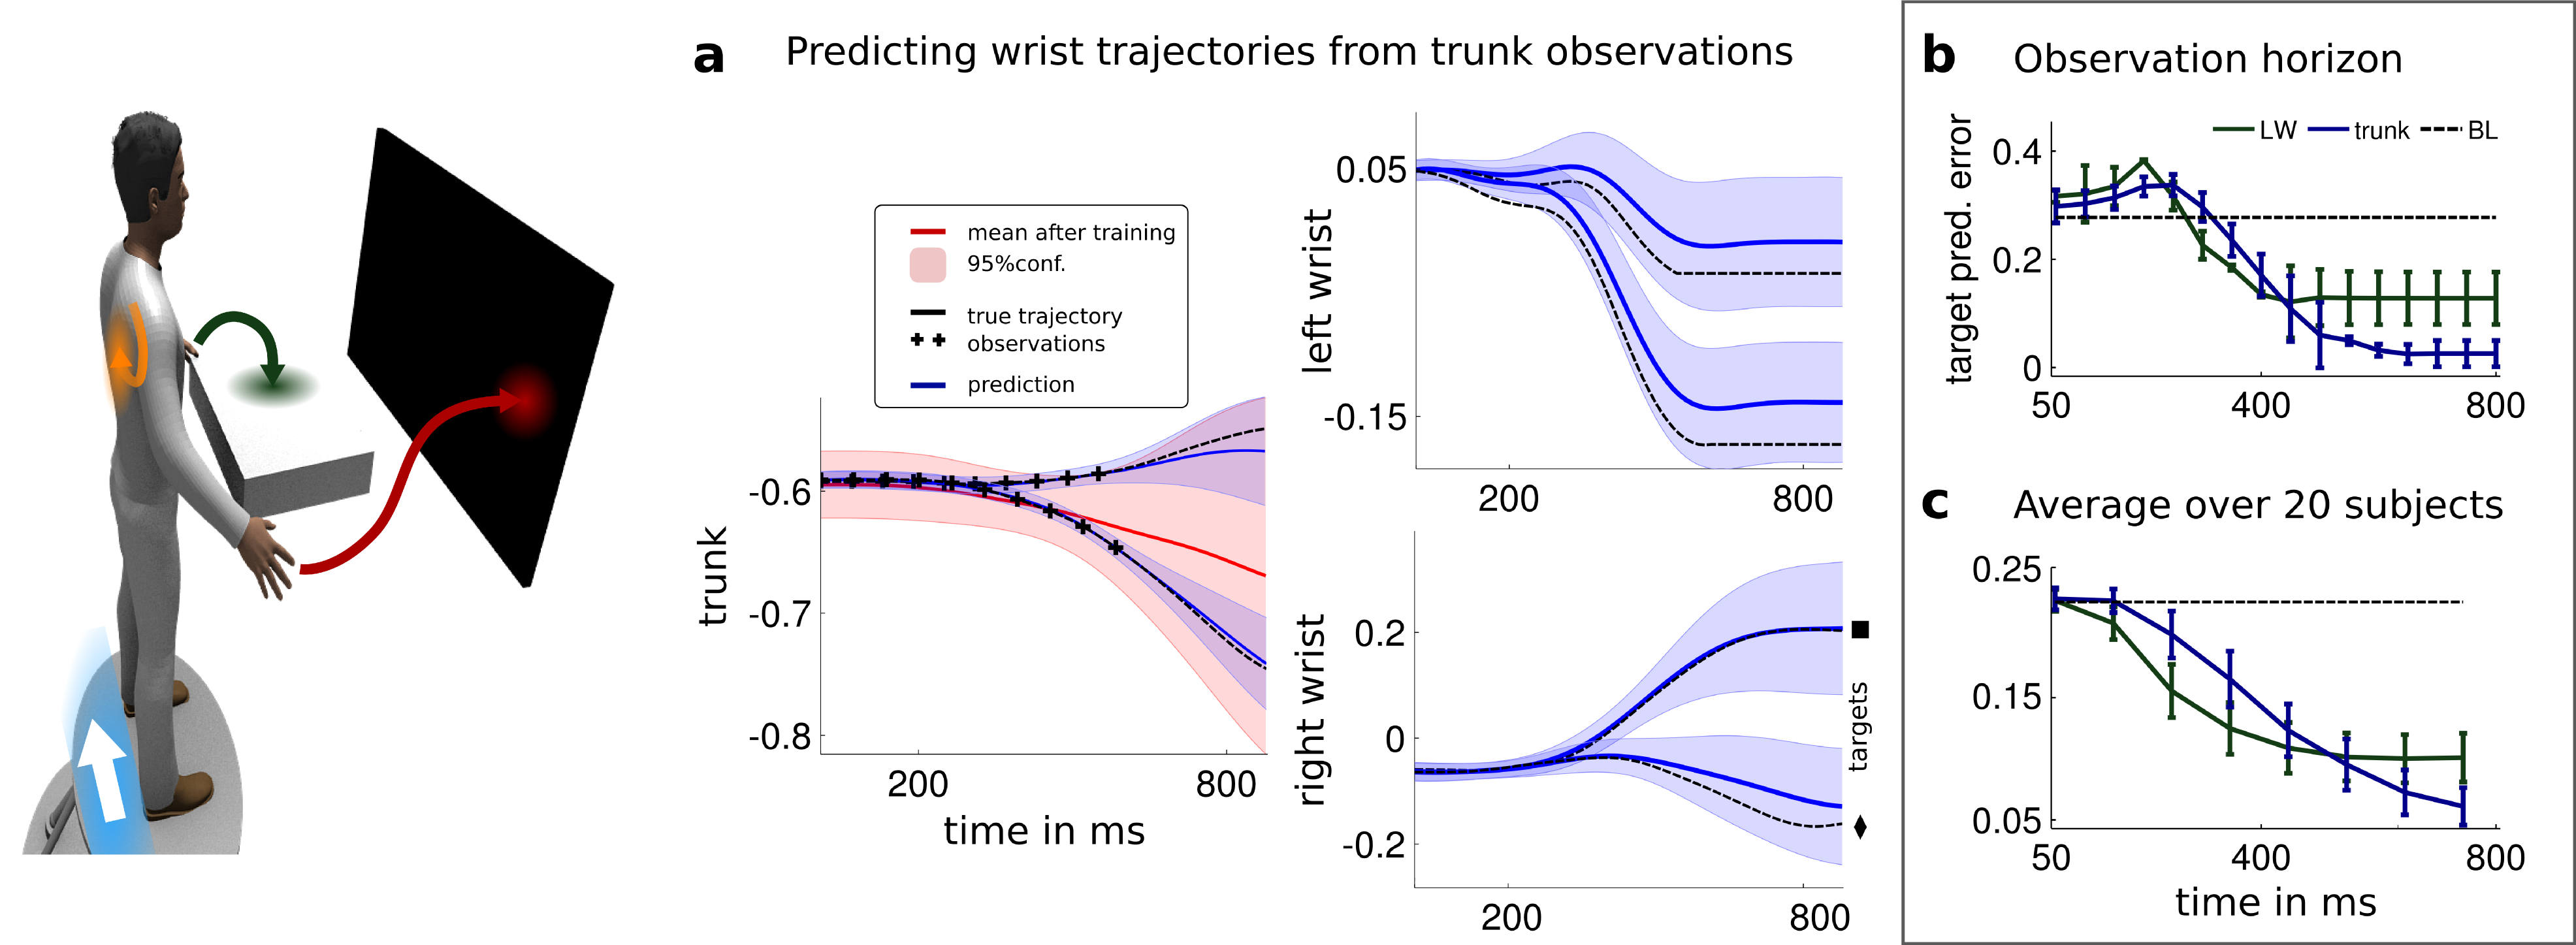
\includegraphics[width=0.8\textwidth]{./sections/WP2/pics_TUD/SummaryFig_Y2Report}
%\label{fig:subfig2}
 \caption{Trunk trajectories predict wrist trajectories.  
 (a) 600ms of trunk trajectories are observed. These observations can predict the wrist trajectories. Shown are predictions for the two exterior targets on the screen. 
 For training 10 trials for each target are used starting from trial 240 backwards in time (before the catch trials). For testing the first perturbed trial after trial number 240 were used. 
 (b) The effect of the observation horizon on the target prediction error is shown for a representative subject. The mean of the training data denotes the base line (BL). (c) Average statistics (mean and 95 percent confidence bound) over 20 subjects.
}
\label{fig:HumanProMPsPrediction}
\end{figure}
In collaboration with JSI, TUD studied whether supporting contacts
in human arm reaching tasks are planned or an effect of a reactive controller. 
Investigations on human motor learning has focused on adaptation experiments with fixed contact points leaving 
research on the computational role of contacts as a free control variable unexplored. 
In perturbed target reaching experiments sketched in Figure \ref{fig:HumanProMPsPrediction}, we studied weather supporting contacts are planned or reactive. 
Subjects had to reach for distant targets on a screen with their right hand. 
For reaching the target additional support through contacts with a table using the left hand was inevitably. 
If the contacts are planned then the left hand's motion can predict the right hand reaching. 
We studied how probabilistic inference in learned models can be used to answer this question. 
Evidence for planned contacts could be provided through learning probabilistic models of trajectory distributions and using the models to generate predictions, Figure \ref{fig:HumanProMPsPrediction} (a). 
We found that the target on the screen could be predicted from both, the left hand (mse: $10.4$cm $\pm$ $2$cm over $20$ subjects) and the trunk movement (mse: $6.7$cm $\pm$ $1.4$cm over $20$ subjects), which 
is illustrated in Figure \ref{fig:HumanProMPsPrediction} (b-c). 
The learned probabilistic model could also be used to analyse the rate of adaptation of the left hand and the trunk kinematics, 
where the trunk trajectories converged faster than the left hand motion. 
This is intuitively explained by the strong need for corrective trunk movements in balancing. 
A report on the findings is currently in progress of writting.

